\textbf{Chapter 12: Weak Interactions of Leptons}

Lepton Universality: $G_F^{(e)} = G_F^{(\mu)} = G_F^{(\tau)}$ (within experimental error)

Neutrino-quark scattering:

$M_{fi} = \frac{g_W^2}{2m_W^2} g_{\mu\nu}\left[\bar{u}(p_3) \gamma^\mu \frac{1}{2}(1 - \gamma^5) u(p_1)\right]\left[\bar{u}(p_4) \gamma^\mu \frac{1}{2}(1 - \gamma^5) u(p_2)\right]$

$\implies \frac{d\sigma_{\nu q}}{d\Omega^*} = \frac{G_F^2}{4\pi^2} \hat{s} \implies \sigma_{\nu q} = \frac{G_F^2\hat{s}}{\pi}$

\begin{center}
    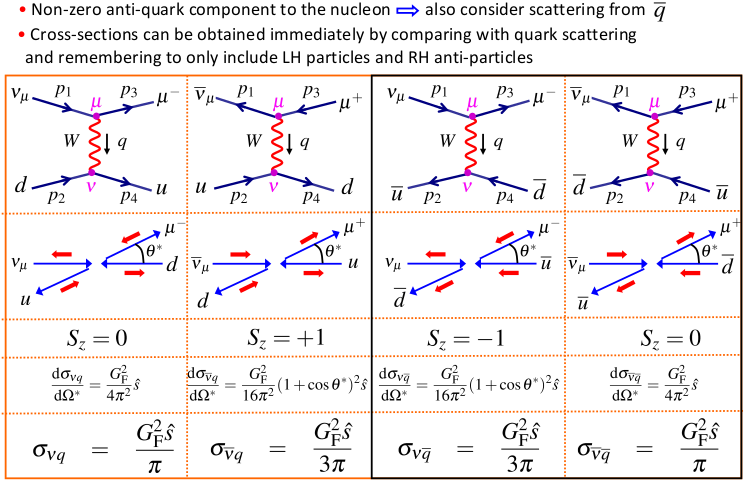
\includegraphics[width=\linewidth]{images/nu_q_scattering.png}
\end{center}

$F_2^{\nu p} = 2xF_1^{\nu p} = 2x[d(x) + \bar{u}(x)]$

$xF_3^{\nu p} = 2x[d(x) - \bar{u}(x)]$

$\sigma^{\nu N} = \frac{G_F^2 m_N E_\nu}{\pi}\left[f_q + \frac{1}{3}f_{\bar{q}}\right], \sigma^{\bar{\nu} N} = \frac{G_F^2 m_N E_{\bar{\nu}}}{\pi}\left[\frac{1}{3}f_q + f_{\bar{q}}\right]$

